\iffalse
\let\negmedspace\undefined
\let\negthickspace\undefined
\documentclass[journal,12pt,twocolumn]{IEEEtran}
\usepackage{cite}
\usepackage{amsmath,amssymb,amsfonts,amsthm}
\usepackage{algorithmic}
\usepackage{graphicx}
\usepackage{textcomp}
\usepackage{xcolor}
\usepackage{txfonts}
\usepackage{listings}
\usepackage{enumitem}
\usepackage{mathtools}
\usepackage{float}
\usepackage{gensymb}
\usepackage{comment}
\usepackage[breaklinks=true]{hyperref}
\usepackage{tkz-euclide} 
\usepackage{listings}
\usepackage{gvv}                                        
\def\inputGnumericTable{}                                 
\usepackage[latin1]{inputenc}                                
\usepackage{color}                                            
\usepackage{array}                                            
\usepackage{longtable}                                       
\usepackage{calc}                                             
\usepackage{multirow}                                         
\usepackage{hhline}                                           
\usepackage{ifthen}                                           
\usepackage{lscape}
\usepackage{amsmath}
\newtheorem{theorem}{Theorem}[section]
\newtheorem{problem}{Problem}
\newtheorem{proposition}{Proposition}[section]
\newtheorem{lemma}{Lemma}[section]
\newtheorem{corollary}[theorem]{Corollary}
\newtheorem{example}{Example}[section]
\newtheorem{definition}[problem]{Definition}
\newcommand{\BEQA}{\begin{eqnarray}}
\newcommand{\EEQA}{\end{eqnarray}}
\newcommand{\define}{\stackrel{\triangle}{=}}
\theoremstyle{remark}
\newtheorem{rem}{Remark}
\begin{document}

\bibliographystyle{IEEEtran}
\title{NCERT 10.5.3.Q20}
\author{EE23BTECH11015 - DHANUSH V NAYAK$^{*}$% <-this % stops a space
}
\maketitle
\newpage
\bigskip
\renewcommand{\thefigure}{\arabic{figure}}
\renewcommand{\thetable}{\theenumi}
\textbf{Question:}In a potato race, a bucket is placed at the starting point, which is 5 m from the first potato,and the other potatoes are placed 3 m apart in a straight line. There are ten potatoes in the line. A competitor starts from the bucket, picks up the nearest potato, runs back with it, drops it in the bucket, runs back to pick up the next potato, runs to the bucket to drop it in, and she continues in the same way until all the potatoes are in the bucket. What is the total distance the competitor has to run?\\
\hfill(NCERT-Maths 10.5.3.20Q)
\begin{figure}[H]
    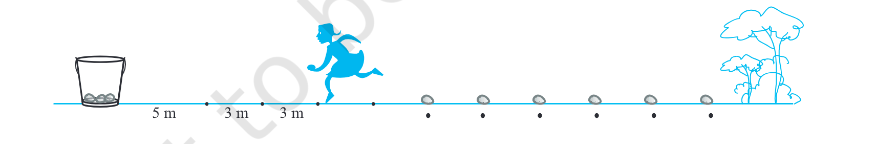
\includegraphics[width=1\columnwidth]{ncert-maths/10/5/3/20/figs/questionfig.png}
    \label{fig:questionfig}
\end{figure}
\solution 
\fi
\begin{table}[H]
\centering
\renewcommand\thetable{1}
\setlength{\extrarowheight}{9pt}
\resizebox{0.5\textwidth}{!}{
\begin{tabular}{|c|c|c|}
\hline
\textbf{Parameter} & \textbf{Description} & \textbf{Value} \\ \hline
$x\brak{0}$ & First term & 10  \\ \hline
$d$ & Common Difference &6 \\ \hline
$y\brak{9}$& Total distance covered  & $?$ \\ \hline 
\end{tabular}}
\caption{Parameter Table}
\label{tab:ncert 10.5.3.20}
\end{table}

From \eqref{eq:apz} :
\begin{align}
    X\brak{z} &= \frac{x(0)}{1-z^{-1}} + \frac{dz^{-1}}{(1-z^{-1})^{2}}, \quad \abs{z} > 1 \\
        &= \frac{10}{1-z^{-1}} + \frac{6z^{-1}}{(1-z^{-1})^{2}}, \quad \abs{z} > 1\\
        &= \frac{10-4z^{-1}}{\brak{1-z^{-1}}^2} \quad \abs{z} > 1 \label{eq:10.5.3.20.1}
\end{align}
From \eqref{eq:conv-sum}
\begin{align}
	y\brak{n} = \sum_{k=0}^{n}x\brak{k} = x(n)*u(n) 
\end{align}

Taking z transform :
\begin{align}
    Y(z) &= X(z) U(z)\\
    \implies Y(z) &=\frac{10-4z^{-1}}{\brak{1-z^{-1}}^3} \quad \abs{z} > 1
\end{align}
Taking inverse z transform :
\begin{align}
    y\brak{n} & =  \frac{1}{2\pi j} \oint_C Y\brak{z} z^{n-1} dz  \\
    y(9)&=\frac{1}{2\pi j}\oint_{C}Y(z) \;z^{8} \;dz  \\
    &=\frac{1}{2\pi j}\oint_{C}\frac{10z^{11}-4z^{10}}{{\brak{z-1}}^{3}} \;dz 
\end{align}
We can observe that the pole is repeated $3$ times and thus $m=3$,
\begin{align}
    R&=\frac{1}{\brak {m-1}!}\lim\limits_{z\to z_{0}}\frac{d^{m-1}}{dz^{m-1}}\brak {f\brak {z}}  \\
    &=\frac{1}{\brak {2}!}\lim\limits_{z\to 1}\frac{d^{2}}{dz^{2}}\brak {10z^{11}-4z^{10}} \\
    &=370
\end{align}
\begin{align}
    \therefore y\brak{9}=370
\end{align}


\begin{figure}[H]
    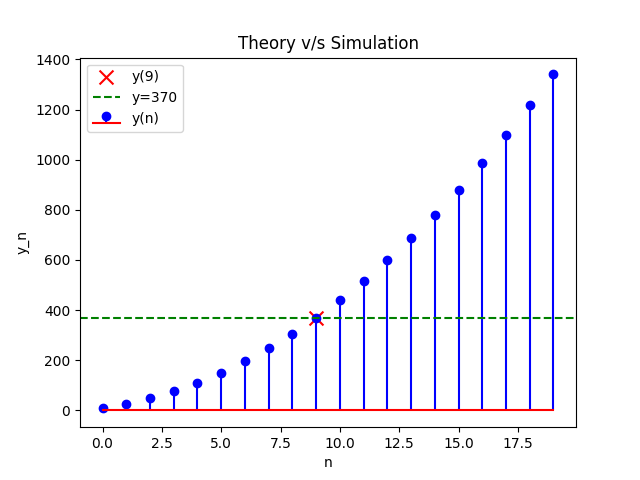
\includegraphics[width=1\columnwidth]{ncert-maths/10/5/3/20/figs/Ncert_10.5.3.20stemplot.png}
    \caption{Theory matches with the simulated values}
    \label{fig:plot10.5.3.20}
\end{figure}


%\end{document}



